% Primary source: https://doi.org/10.1016/S0004-3702(99)00052-1
\documentclass[tikz,border=5pt]{standalone}
\usepackage[T1]{fontenc}
\usepackage{lmodern,amsmath,amssymb}
\usetikzlibrary{arrows.meta,calc,positioning,fit,backgrounds,shapes.geometric,matrix,decorations.pathreplacing,patterns}
\definecolor{ink}{gray}{0.08}
\definecolor{wash}{gray}{0.965}
\definecolor{soft}{gray}{0.45}
\tikzset{box/.style={draw=ink,line width=.65pt,fill=white,align=center,inner sep=4pt,outer sep=0pt,font=\small},flow/.style={draw=ink,line width=.65pt,-{Latex[length=1.8mm,width=1.3mm]},rounded corners=2pt},annotation/.style={font=\scriptsize,text=soft,align=center},groupbox/.style={draw=soft,dashed,line width=.45pt,fill=wash}}
\begin{document}
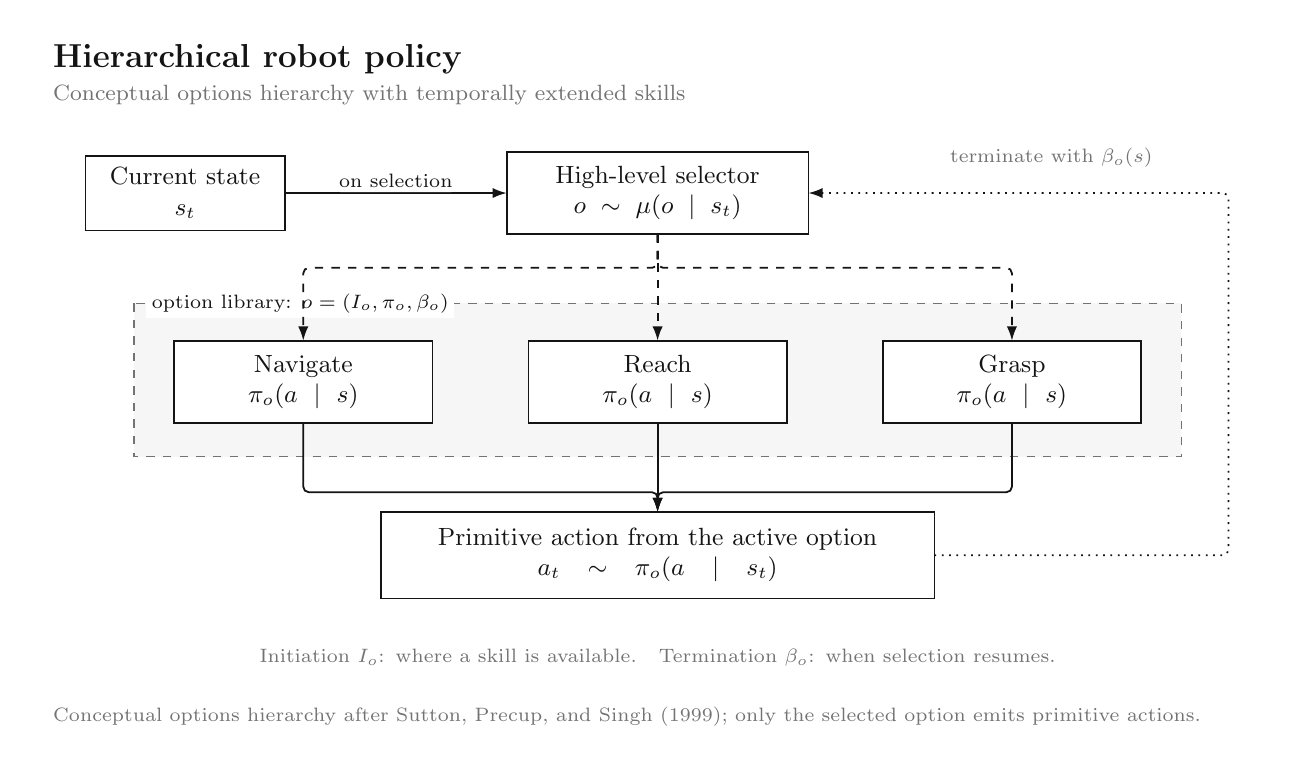
\begin{tikzpicture}[x=1cm,y=-1cm,font=\rmfamily,text=ink]

\path[use as bounding box] (0,0) rectangle (16,9);
\node[anchor=west,font=\large\bfseries] at (.2,.4) {Hierarchical robot policy};
\node[anchor=west,font=\footnotesize,text=soft] at (.2,.85) {Conceptual options hierarchy with temporally extended skills};
\begin{pgfonlayer}{background}
\draw[groupbox] (1.35,3.5) rectangle (14.65,5.45);
\node[anchor=west,font=\scriptsize,fill=white,inner sep=2pt] at (1.5,3.5) {option library: $o=(I_o,\pi_o,\beta_o)$};
\end{pgfonlayer}
\node[box,minimum width=2.5cm,minimum height=0.95cm,text width=2.25cm] (state) at (2.0,2.1) {Current state\\$s_t$};
\node[box,minimum width=3.8cm,minimum height=1.05cm,text width=3.55cm] (selector) at (8.0,2.1) {High-level selector\\$o\sim\mu(o\mid s_t)$};
\node[box,minimum width=3.25cm,minimum height=1.05cm,text width=3.0cm] (nav) at (3.5,4.5) {Navigate\\$\pi_o(a\mid s)$};
\node[box,minimum width=3.25cm,minimum height=1.05cm,text width=3.0cm] (reach) at (8.0,4.5) {Reach\\$\pi_o(a\mid s)$};
\node[box,minimum width=3.25cm,minimum height=1.05cm,text width=3.0cm] (grasp) at (12.5,4.5) {Grasp\\$\pi_o(a\mid s)$};
\node[box,minimum width=7.0cm,minimum height=1.1cm,text width=6.75cm] (primitive) at (8.0,6.7) {Primitive action from the active option\\$a_t\sim\pi_o(a\mid s_t)$};
\begin{pgfonlayer}{background}
\draw[flow,dashed] (selector.south) -- (8.0,3.05) -- (3.5,3.05) -- (nav.north);
\draw[flow,dashed] (selector.south) -- (8.0,3.05) -- (8.0,3.05) -- (reach.north);
\draw[flow,dashed] (selector.south) -- (8.0,3.05) -- (12.5,3.05) -- (grasp.north);
\draw[flow] (state.east) -- (selector.west) node[midway,above,fill=white,inner sep=1.5pt,font=\scriptsize] {on selection};
\draw[flow] (nav.south) -- (3.5,5.9) -- (8.0,5.9) -- (primitive.north);
\draw[flow] (reach.south) -- (8.0,5.9) -- (8.0,5.9) -- (primitive.north);
\draw[flow] (grasp.south) -- (12.5,5.9) -- (8.0,5.9) -- (primitive.north);
\draw[flow,dotted] (primitive.east) -- (15.25,6.7) -- (15.25,2.1) -- (selector.east);
\end{pgfonlayer}
\node[annotation,text width=4.1cm] at (13.0,1.65) {terminate with $\beta_o(s)$};
\node[annotation,text width=13.2cm] at (8.0,8.0) {Initiation $I_o$: where a skill is available.\quad Termination $\beta_o$: when selection resumes.};
\node[anchor=west,align=left,font=\scriptsize,text=soft,text width=15.6cm] at (.2,8.75) {Conceptual options hierarchy after Sutton, Precup, and Singh (1999); only the selected option emits primitive actions.};
\end{tikzpicture}
\end{document}
